\section{Monte Carlo Simulations}

Monte Carlo methods belongs to a category of computational algorithms that
utilize repeated random sampling to derive numerical outcomes. These methods are
extensively employed across various fields such as physics, chemistry, and
finance. In this thesis, Monte Carlo methods are specifically applied to
simulate the Ising model.

The Ising model is characterized as a stochastic system, meaning its behavior is
inherently probabilistic rather than deterministic. In such a system, the state
at any given moment is subject to random variation, making precise prediction
unfeasible. This contrasts with deterministic systems, where, provided the
initial conditions and the governing rules are known, the future state of the
system can be accurately forecasted.

In the context of the Ising model, stochasticity arises primarily from thermal
fluctuations. These fluctuations spontaneously induce spin reversals, leading to
unpredictable variations in the system's energy state. Consequently, the
evolution of the system's state over time remains indeterminable.

Given these characteristics, the Monte Carlo method emerges as an apt approach
for simulating systems like the Ising model, where randomness plays a pivotal
role in their evolution.

For this thesis, the goal of the Monte Carlo simulation is to estimate the
expectation values:

\begin{equation}
\langle \mathcal{O} \rangle \equiv \sum_{\text{states } \sigma} \mathcal{O}(\sigma) e^{-\beta \mathcal{H}(\sigma)} / \mathcal{Z}
\end{equation}

where $\mathcal{O}$ is an observable of the system defined by its Hamiltonian
$\mathcal{H}$ and with canonical partition function $\mathcal{Z}$ as:

\begin{equation}
\mathcal{Z} = \sum_{\text{states } \sigma} e^{-\beta \mathcal{H}(\sigma)} = \sum_{E} \Omega(E) e^{-\beta E}
\end{equation}

where $\Omega(E)$ is the density of states at energy $E$.

\subsection{Importance Sampling and Markov Chain Monte Carlo Methods}

Importance sampling is a Monte Carlo technique that enhances the efficiency of
simulations by reducing the variance of estimated expectation values. This
technique involves drawing samples not randomly but in accordance with a
specified equilibrium distribution. In many physical systems, this equilibrium
distribution is defined by the canonical ensemble's Boltzmann weight, expressed
as 

\begin{equation}
    \mathcal{P}^{eq}_i \equiv \mathcal{P}^{eq}(\sigma_i) = \frac{e^{-\beta H(\sigma_i)}}{Z}
\end{equation}
although the principle of importance sampling is not restricted to this
particular form.

In the context of Markov Chain Monte Carlo (MCMC) methods, a Markov chain is
established to select a microstate \( \sigma_i \) according to the given
equilibrium distribution. A Markov chain is characterized by its transition
probabilities \( W_{ij} \equiv W(\sigma_i \rightarrow \sigma_j) \), which
dictate the likelihood of a system evolving from one microstate \( \sigma_i \)
to another \( \sigma_j \). This evolution is subject to the condition that the
probability depends only on the current state \( \sigma_i \) and not on the
entire history of the system's trajectory, rendering the process almost local in
time.

For MCMC algorithms to accurately reflect the equilibrium distribution, the
transition probability \( W_{ij} \) must satisfy three conditions:

\begin{enumerate}
    \item \( W_{ij} \geq 0 \qquad \forall i, j \) (positivity),
    \item \( \sum_j W_{ij} = 1  \qquad \forall i \) (normalization),
    \item \( \sum_i W_{ij} \mathcal{P}^{eq}_i = \mathcal{P}^{eq}_j \qquad
    \forall j \) (balance condition).
\end{enumerate}

The balance condition ensures that the equilibrium distribution is a fixed point
of the transition matrix \( W \), maintaining the desired distribution across
the Markov chain. A commonly used strategy to satisfy this condition is the
detailed balance, which states that \( W_{ij} P^{eq}_i = W_{ji} P^{eq}_j \).
This condition, when combined with normalization, ensures the general balance
condition.

After an initial equilibration period, expectation values in the system can be
estimated as the arithmetic mean over the Markov chain. This means calculating
the average of a quantity \( \mathcal{O} \) over different states of the system,
represented as follows:

\begin{equation}
    \langle \mathcal{O} \rangle = \sum_{\sigma}\mathcal{O}(\sigma)\mathcal{P}^{eq}(\sigma) \approx \overline{\mathcal{O}} \equiv \frac{1}{N} \sum_{k=1}^{N}\mathcal{O}(\sigma(k))
\end{equation}

where \( \sigma(k) \) denotes the state of the system at step \( k \) in the
Markov chain. This approach provides an unbiased estimator
$\overline{\mathcal{O}} $ for the expectation value \( \langle \mathcal{O}
\rangle \), thus effectively capturing the equilibrium behavior of the system.

\subsection{Local Update Algorithms}

The Markov chain conditions outlined above are general and can be satisfied by a
variety of algorithms. In the context of the Ising model, the Metropolis
algorithm is a widely used local update algorithm that satisfies the conditions
and is therefore suitable for Monte Carlo simulations.

Local update algorithms are characterized by their ability to update the system
by changing only a small portion of the lattice. This is in contrast to global
update algorithms, which require the entire lattice to be updated at each step.
Local update algorithms are more efficient than global update algorithms, as
they require less computational resources to simulate the system.

The selection of a local update algorithm is not arbitrary. The algorithm must
satisfy the detailed balance condition, which is a necessary condition for
achieving the equilibrium distribution. The Metropolis algorithm is one such
algorithm that satisfies this condition. The probability of a potential
transition from state \( \sigma_i \) to \( \sigma_j \) is given by the so called
selection probability \( f_{ij} \), which is defined as:

\begin{equation}
    f_{ij} = f(\sigma_i \rightarrow \sigma_j), \qquad f_{ii} \geq 0, \qquad \sum_j f_{ij} = 1
\end{equation}

The proposed transition is then accepted with the probability \( w_{ij} \),
defined as:

\begin{equation}
    w_{ij} = w(\sigma_i \rightarrow \sigma_j) = \min \left( 1, \frac{f_{ji} \mathcal{P}^{eq}_i}{f_{ij} \mathcal{P}^{eq}_j} \right)
\end{equation}

where \( \mathcal{P}^{eq}_i \) is the equilibrium probability of the state.
Otherwise, the system remains in the same state which may also happen when \(
f_{i} \neq 0 \).

This implies that the transition probability \( W_{ij} \) is given by:

\begin{equation}
    W_{ij} =
    \begin{cases}
        f_{ij} w_{ij} & j \neq i \\
        f_{ii} + \sum_{j \neq i} f_{ij} w_{ij} & j = i
    \end{cases}
\end{equation}

As $f_{ij} \geq 0$ and $0 \leq w_{ij} \leq 1$, it follows that $W_{ij} \geq 0$
and $\sum_j W_{ij} = 1$, satisfying the Markov chain conditions.

The update prescription is still general, as the probability \( \mathcal{P}^{ij}
\) can be chosen arbitrarily. Moreover, the selection probability \( f_{ij} \)
can be chosen to be symmetric, i.e. \( f_{ij} = f_{ji} \), which is the case for
our simulations and it has not been specified how to choose the trail state \(
\sigma_j \). After simplification, the Boltzmann weight from the importance
sampling is obtained which results in:

\begin{equation}
    \frac{\mathcal{P}_j^{eq}}{\mathcal{P}_i^{eq}} = e^{-\beta \Delta E}
\end{equation}

where \( \Delta E = E_j - E_i \) is the energy difference between the two
states.

\subsection{Metropolis Algorithm}

The Metropolis Algorithm was first introduced by Nicholas Metropolis in 1953,
revolutionizing the simulation of stochastic systems. It has since found
extensive applications in diverse fields, including physics, chemistry, and
biology, with a notable impact on the study of the Ising model.

This algorithm falls under the category of Markov chain Monte Carlo (MC MC)
methods. It generates a Markov chain, ensuring that its stationary distribution
aligns with the target probability distribution. In the Ising model, this
entails creating a sequence of spin configurations, each derived from its
predecessor, converging towards the Boltzmann distribution: the equilibrium
probability distribution for the model.

The Metropolis algorithm operates on a rejection-based principle. It involves
the following steps:

\begin{enumerate}
\item Initialize the system with a random spin configuration.
\item Randomly select a spin within the lattice.
\item Compute the energy change, $\Delta E$, resulting from the inversion of the
selected spin.
\item Accept the new configuration if $\Delta E < 0$.
\item For $\Delta E > 0$, accept the new configuration with a probability of
$e^{-\beta \Delta E}$.
\item Iterate steps 2-5 until a predetermined number of iterations is achieved.
\end{enumerate}

The Metropolis algorithm's simplicity and efficacy make it an ideal tool for
simulating the Ising model. Its versatility allows for adaptations to different
scenarios, such as varying the temperature in the Ising model simulations by
adjusting the acceptance probability in the algorithm.

Based on above steps, the acceptance probability is given by:

\begin{equation}
    w_{ij} = \min \left( 1, \frac{f_{ji} \mathcal{P}^{eq}i}{f{ij} \mathcal{P}^{eq}_j} \right) \\
    = \min \left( 1, e^{-\beta \Delta E} \right) \\
    =
    \begin{cases}
        1 & \text{if } \Delta E \leq 0, \\
        e^{-\beta \Delta E} & \text{if } \Delta E > 0.
    \end{cases}
\end{equation}

\begin{figure}
    \centering
    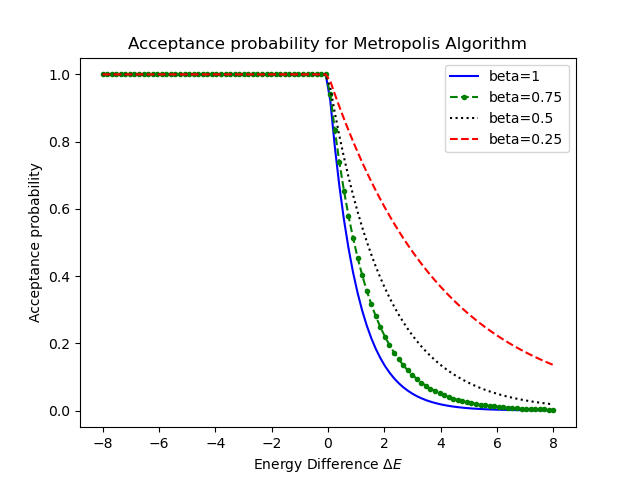
\includegraphics[width=0.8\textwidth]{images/metropolis.png}
    \caption{The Metropolis algorithm for the Ising model.}
    \label{fig:metropolis}
\end{figure}

If the energy difference is negative, the new state is always accepted. If the
energy difference is positive, the new state is accepted with a probability
defined in the equation above. This is illustrated in Figure
\ref{fig:metropolis}. This ensures the proper treatment of entropic
contributions in thermal equilibrium. The free energy, $F = U -TS $ has to be
minimized and not the internal energy $U$.

For the Ising model with only two possible spin states, a spin flip is the only
possible local update. This means that the selection probability \( f_{ij} \) is
symmetric, i.e. \( f_{ij} = f_{ji} \). The selection probability is also
independent of the state \( \sigma_i \) and \( \sigma_j \), i.e. \( f_{ij} =
f_{ji} = f_{i} \). This implies that the transition probability \( W_{ij} \) is
given by:

\begin{equation}
    W_{ij} =
    \begin{cases}
        f_{ij} w_{ij} & j \neq i \\
        f_{ii} + \sum_{j \neq i} f_{ij} w_{ij} & j = i
    \end{cases}
\end{equation}

The update prescription is still general, as the probability \( \mathcal{P}^{ij}
\) can be chosen arbitrarily. Moreover, the selection probability \( f_{ij} \)
can be chosen to be symmetric, i.e. \( f_{ij} = f_{ji} \), which is the case for
our simulations. To decide whether the proposed transition is accepted or not,
we draw a random number \( r \) from a uniform distribution between 0 and 1. If
\( r \leq w_{ij} \), the transition is accepted, otherwise it is rejected and we
continue with next step in the Markov chain.
